% Architecture diagram for Mamba3Yolo
% Can be \input{} into main.tex or compiled standalone
% Compile: pdflatex architecture.tex  (or use \includegraphics after converting)

\documentclass[tikz,border=8pt]{standalone}
\usepackage{tikz}
\usetikzlibrary{positioning, arrows.meta, fit, calc, backgrounds, shadows.blur}
\usepackage{xcolor}

% Colors
\definecolor{stemC}{RGB}{70,130,180}
\definecolor{mambaC}{RGB}{220,80,60}
\definecolor{lsC}{RGB}{60,160,90}
\definecolor{rgC}{RGB}{240,160,40}
\definecolor{neckC}{RGB}{120,90,180}
\definecolor{headC}{RGB}{50,50,50}
\definecolor{lightgray}{RGB}{245,245,245}
\definecolor{boxbg}{RGB}{255,255,255}

\begin{document}
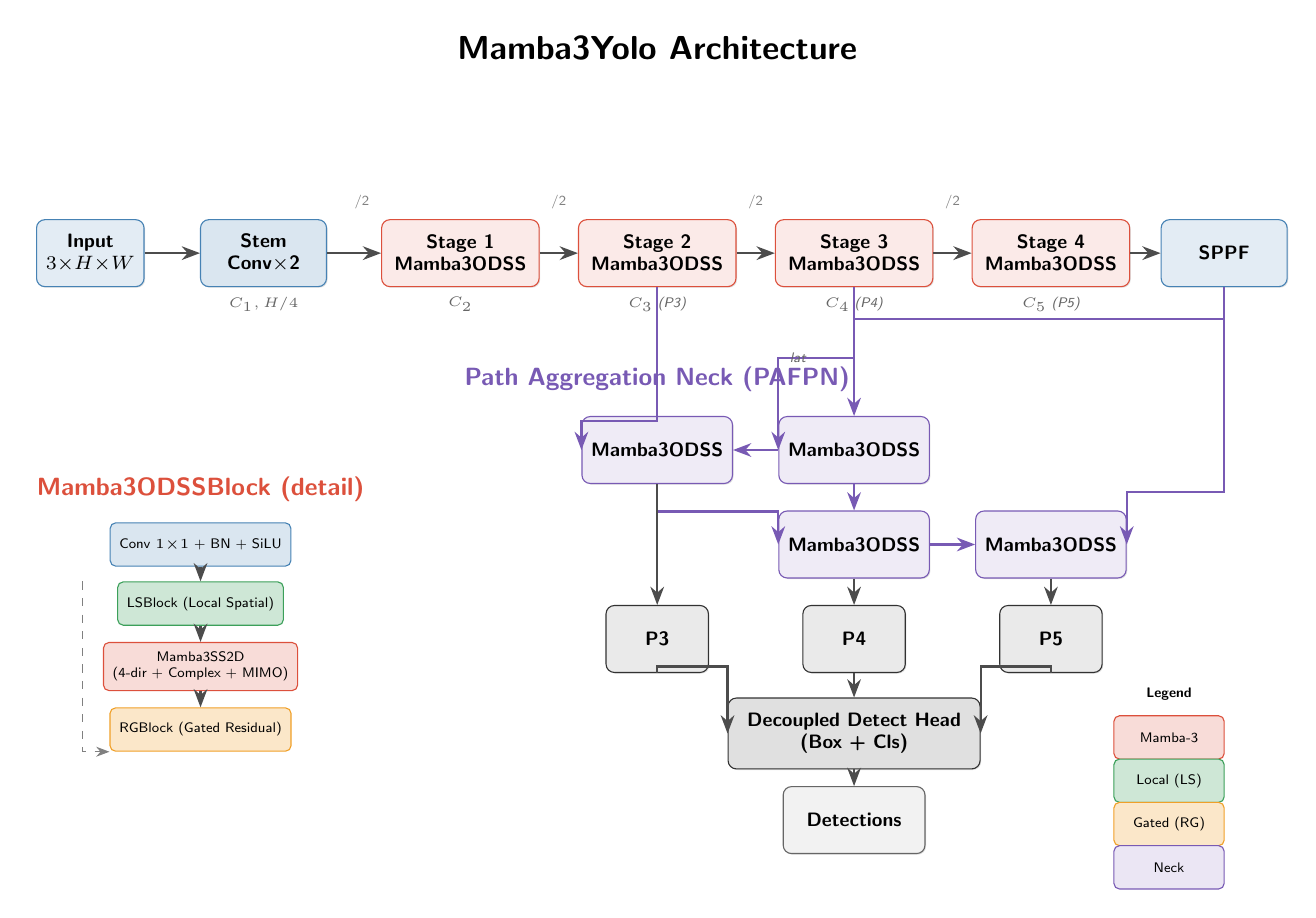
\begin{tikzpicture}[
    font=\sffamily\footnotesize,
    >=Stealth,
    block/.style={
        draw, rounded corners=3pt, align=center,
        minimum height=0.85cm, minimum width=1.6cm,
        fill=boxbg, drop shadow={shadow xshift=0.4pt, shadow yshift=-0.4pt, opacity=0.25},
        font=\sffamily\scriptsize\bfseries
    },
    smallblock/.style={
        draw, rounded corners=2pt, align=center,
        minimum height=0.55cm, minimum width=1.15cm,
        fill=boxbg, font=\sffamily\tiny
    },
    arrow/.style={->, thick, color=black!70},
    label/.style={font=\sffamily\tiny\itshape, text=black!60},
    stage/.style={font=\sffamily\tiny, text=black!50}
]

% ========== TITLE ==========
\node[font=\sffamily\large\bfseries] at (0, 5.8) {Mamba3Yolo Architecture};

% ========== INPUT ==========
\node[block, fill=stemC!15, draw=stemC, minimum width=1.3cm] (input) at (-7.2, 3.2) {Input\\$3{\times}H{\times}W$};

% ========== STEM ==========
\node[block, fill=stemC!20, draw=stemC] (stem) at (-5.0, 3.2) {Stem\\Conv$\times$2};

% ========== BACKBONE STAGES ==========
\node[block, fill=mambaC!12, draw=mambaC, minimum width=2.0cm] (s1) at (-2.5, 3.2) {Stage 1\\Mamba3ODSS};
\node[block, fill=mambaC!12, draw=mambaC, minimum width=2.0cm] (s2) at (0.0, 3.2) {Stage 2\\Mamba3ODSS};
\node[block, fill=mambaC!12, draw=mambaC, minimum width=2.0cm] (s3) at (2.5, 3.2) {Stage 3\\Mamba3ODSS};
\node[block, fill=mambaC!12, draw=mambaC, minimum width=2.0cm] (s4) at (5.0, 3.2) {Stage 4\\Mamba3ODSS};

\node[block, fill=stemC!15, draw=stemC] (sppf) at (7.2, 3.2) {SPPF};

% Downsample labels
\node[stage] at (-3.75, 3.85) {/2};
\node[stage] at (-1.25, 3.85) {/2};
\node[stage] at (1.25, 3.85) {/2};
\node[stage] at (3.75, 3.85) {/2};

% Arrows backbone
\draw[arrow] (input) -- (stem);
\draw[arrow] (stem) -- (s1);
\draw[arrow] (s1) -- (s2);
\draw[arrow] (s2) -- (s3);
\draw[arrow] (s3) -- (s4);
\draw[arrow] (s4) -- (sppf);

% Feature map sizes
\node[label] at (-5.0, 2.55) {$C_1, H/4$};
\node[label] at (-2.5, 2.55) {$C_2$};
\node[label] at (0.0, 2.55) {$C_3$ (P3)};
\node[label] at (2.5, 2.55) {$C_4$ (P4)};
\node[label] at (5.0, 2.55) {$C_5$ (P5)};

% ========== NECK (PAFPN) ==========
\node[font=\sffamily\small\bfseries, text=neckC] at (0, 1.6) {Path Aggregation Neck (PAFPN)};

% Top-down
\node[block, fill=neckC!12, draw=neckC, minimum width=1.7cm] (n1) at (2.5, 0.7) {Mamba3ODSS};
\node[block, fill=neckC!12, draw=neckC, minimum width=1.7cm] (n2) at (0.0, 0.7) {Mamba3ODSS};

% Bottom-up
\node[block, fill=neckC!12, draw=neckC, minimum width=1.7cm] (n3) at (2.5, -0.5) {Mamba3ODSS};
\node[block, fill=neckC!12, draw=neckC, minimum width=1.7cm] (n4) at (5.0, -0.5) {Mamba3ODSS};

% Lateral / upsample arrows
\draw[arrow, neckC] (sppf.south) -- ++(0,-0.4) -| (n1.north);
\draw[arrow, neckC] (s3.south) -- ++(0,-0.9) -| node[pos=0.25, left, label] {lat} (n1.west);
\draw[arrow, neckC] (n1) -- (n2);
\draw[arrow, neckC] (s2.south) -- ++(0,-1.7) -| (n2.west);

\draw[arrow, neckC] (n2.south) -- ++(0,-0.35) -| (n3.west);
\draw[arrow, neckC] (n1.south) -- (n3.north);
\draw[arrow, neckC] (n3) -- (n4);
\draw[arrow, neckC] (sppf.south) -- ++(0,-2.6) -| (n4.east);

% Outputs
\node[block, fill=headC!10, draw=headC, minimum width=1.3cm] (p3) at (0.0, -1.7) {P3};
\node[block, fill=headC!10, draw=headC, minimum width=1.3cm] (p4) at (2.5, -1.7) {P4};
\node[block, fill=headC!10, draw=headC, minimum width=1.3cm] (p5) at (5.0, -1.7) {P5};

\draw[arrow] (n2.south) -- (p3.north);
\draw[arrow] (n3.south) -- (p4.north);
\draw[arrow] (n4.south) -- (p5.north);

% ========== HEAD ==========
\node[block, fill=headC!15, draw=headC, minimum width=3.2cm, minimum height=0.9cm] (head) at (2.5, -2.9) {Decoupled Detect Head\\(Box + Cls)};

\draw[arrow] (p3) -- ++(0,-0.35) -| (head.west);
\draw[arrow] (p4) -- (head.north);
\draw[arrow] (p5) -- ++(0,-0.35) -| (head.east);

\node[block, fill=black!5, draw=black!60, minimum width=1.8cm] (out) at (2.5, -4.0) {Detections};

\draw[arrow] (head) -- (out);

% ========== ZOOM: Mamba3ODSSBlock ==========
\begin{scope}[shift={(-5.8,-1.8)}]
    \node[font=\sffamily\small\bfseries, text=mambaC] at (0, 2.0) {Mamba3ODSSBlock (detail)};
    
    \node[smallblock, fill=stemC!20, draw=stemC] (b1) at (0, 1.3) {Conv $1{\times}1$ + BN + SiLU};
    \node[smallblock, fill=lsC!25, draw=lsC] (b2) at (0, 0.55) {LSBlock (Local Spatial)};
    \node[smallblock, fill=mambaC!20, draw=mambaC, minimum width=2.4cm] (b3) at (0, -0.25) {Mamba3SS2D\\(4-dir + Complex + MIMO)};
    \node[smallblock, fill=rgC!25, draw=rgC] (b4) at (0, -1.05) {RGBlock (Gated Residual)};
    
    \draw[arrow] (b1) -- (b2);
    \draw[arrow] (b2) -- (b3);
    \draw[arrow] (b3) -- (b4);
    
    % residual indicators
    \draw[->, dashed, gray] ([xshift=-1.5cm]b2.north) |- ([xshift=-1.5cm]b4.south) -- (b4.south west);
\end{scope}

% ========== LEGEND ==========
\begin{scope}[shift={(6.5,-3.5)}]
    \node[font=\sffamily\tiny\bfseries] at (0, 1.1) {Legend};
    \node[smallblock, fill=mambaC!20, draw=mambaC, minimum width=1.4cm] at (0, 0.55) {Mamba-3};
    \node[smallblock, fill=lsC!25, draw=lsC, minimum width=1.4cm] at (0, 0.0) {Local (LS)};
    \node[smallblock, fill=rgC!25, draw=rgC, minimum width=1.4cm] at (0, -0.55) {Gated (RG)};
    \node[smallblock, fill=neckC!15, draw=neckC, minimum width=1.4cm] at (0, -1.1) {Neck};
\end{scope}

\end{tikzpicture}
\end{document}
